\documentclass[a4paper,12pt]{article} 
\usepackage{amsmath,amssymb, amsthm, mathrsfs, fancyhdr, ulem, gastex, gensymb, harmony, color, enumitem, bm, hyperref, extarrows, makeidx, rotating, wasysym}
\usepackage[encapsulated]{CJK}
\usepackage{ucs}
\usepackage[utf8x]{inputenc}
% use one of bsmi(trad Chinese), gbsn(simp Chinese), min(Japanese), mj(Korean); see:
% /usr/share/texmf-dist/tex/latex/cjk/texinput/UTF8/*.fd
\usepackage{tikz} 
\usetikzlibrary{arrows,decorations.pathmorphing,backgrounds,fit}  
\newcommand\independent{\protect\mathpalette{\protect\independenT}{\perp}} 
\def\independenT#1#2{\mathrel{\rlap{$#1#2$}\mkern2mu{#1#2}}} 


\pdfpagewidth 8.5in
\pdfpageheight 11in
\setlength\topmargin{0in}
\setlength\headheight{0in}
\setlength\headsep{0in}
\setlength\textheight{9.0in}
\setlength\textwidth{6.5in}
\setlength\oddsidemargin{0in}
\setlength\evensidemargin{0in}
\setlength\parindent{0.0in}
\setlength\parskip{0.25in} 

\pagestyle{fancy}
\headheight 15pt
\headsep 20pt

\def\newop#1 
{\expandafter\def\csname #1 
\endcsname{\mathop{\rm #1}\nolimits}} 
%Use as \newop{Blah}, then \Blah works. Similar to say, \dim, or \min, etcc

\lhead[A1 Report \thepage]{Ben Athiwaratkun and Keegan Kang} 
\rhead[Ben Athiwaratkun and Keegan Kang]{A1 Report \thepage} 	
\chead{}
\cfoot{}

\newtheorem{theorem}{Theorem}[section]
\newtheorem{lemma}{Lemma}[section]
\newtheorem{proposition}{Proposition}[section]
\newtheorem{corollary}{Corollary}[section]
\newtheorem{definition}{Definition}[section]
\newtheorem{example}{Example}[section]
\newtheorem{exercise}{Exercise}[section]
\newtheorem{fact}{Fact}[section]
\newtheorem{question}{Question}[section]
\newtheorem{process}{Process}[section]
\newtheorem{skill}{Skill}[section]
\newtheorem{result}{Result}[section]
\newtheorem{remark}{Remark}[section]
\numberwithin{equation}{section}
\newcommand{\cntext}[1]{\begin{CJK}{UTF8}{gbsn}#1\end{CJK}}

\makeindex
\begin{document} 

\subsubsection*{Introduction}

% TODO 
% organize proposed techniques
% include plots for comment lengths in threads (if useful)
% 


Many goals in NLP focus on analyzing a chunk of text, and making some sort of prediction or identification about it. In the CS6742 course, we were given two articles \cite{dejareview} and \cite{anae} to read, and come up with interesting research proposals. 

\cite{anae} acknowledges the failure of traditional moderation methods in ensuring productive conversation on forum posts and threads. The article explores changes to traditional moderation systems, and puts forth the idea of evaluating conversations in threads as an indicator of engagement within the online community, instead of just looking at comments.

While several interesting research questions were proposed, we will only look at the following problem.

\subsubsection*{Research problem}

The problem is stated as such: {\it Can we predict the dynamics of any two active users, based on their previous posts?}

Our analysis will be done using data from BC3's blog corpus, in particular the Slashdot blog conversations. Using this data, we would like to answer the following questions:
\vspace*{-0.5cm}
\begin{enumerate}
%\item We would like to know if we can predict the length of a thread, given two particular users drawn from the top $k$ posters\footnote{Here, the top $k$ posters refer to users with the top $k$ number of posts.}.
\item We would like to know if we can predict the trend of a thread, given the earliest $k$ comments in the article. The trend here can be the length, a moderation class, the moderation score, or some derived feature based on the text such as aggressiveness, politeness, etc. 
\item Given the probability distribution ${\bf p}_A = ({p_1}_A, {p_2}_A,\hdots, {p_n}_A)$ for any user $A$ to create posts of quality $1,2,\hdots, n$, we would like to estimate the conditional probability vector ${\bf p}_{A|\mathcal E}$ of user $A$, given that some event $\mathcal E$ has occurred. Here, $\mathcal E$ could be a shift in topic of the thread, or the entry of a new user.
\end{enumerate}
%Both questions which fall under the umbrella of our research problem.

%Here, we will first look at seeing if it is possible to predict the number of comments a particular thread receives based on the first few posts, as well as how productive a thread could be.


%modify and expound on forum - use LL's 1a) / 1b)

\subsubsection*{Proposed techniques and processing and selection of data}
\begin{enumerate}
\item We analyze the data to prepare for research question 1 by looking at the frequencies of moderation classes. 

\item We plot the comment length in each thread to see if there are any discernible patterns. We represent a thread as a collection of all comments sorted chronologically. An alternative could be to represent a single thread as a path from root to leaf. 

\item To address research question 2, we consider the distribution of the comment length for a given user and compare it with the conditional distribution of comment length of the same user conditioned that another user having posted at least once in the thread. 
\end{enumerate}



%Therefore, we will need to find a way to categorize the {\tt None} comments. One idea of ours is to compute several metrics, such as those in the handout \cite{Otterbacher}\footnote{While these metrics refer to reviews in particular, we will consider metrics 8-17.}, from all the comments. We then see if we can utilize a classification algorithm, such as the $k$-nearest neighbors to classify the other {\tt None:} comments.

\cite{Backstrom+al:13a} also proposes a metric based on whether two users are connected to each other\footnote{This study looks at Facebook and Wikipedia editors. Facebook users are connected if they are mutual friends, and Wikipedia editors are connected if one an editor posted on another editor's page.}. Although there is nothing similar to that for the Slashdot data, we propose a metric of the following: We take a look at the datestamps of the posts of any two particular users, and construct an interval around each datestamp, and assume that this is a user's available time online. We take the ratio of the intersection of two users' available time to their total time to be a metric\footnote{For example, if user $a$ has the time intervals $T_1 \cup T_2 \cup \hdots \cup T_n = A$, and user $b$ has the time intervals $T'_1, \cup T'_2 \cup \hdots \cup T'_m = B$, we would look at the ratio $\frac{A \cap B}{A \cup B}$. }. 

We hope that we can use these metrics to eventually classify the rest of the {\tt None} posts. Then, we can then look at the empirical probability and conditional probability, and do more analysis of the data.

Ideally, we would like to use the entire Slashdot blog corpus and split it into a testing and training set, but it is highly possible that some comments will be hard to classify, and we might have to discard them.


%\cite{Backstrom+al:13a} and 


%As we are using data from Slashdot conversations, the techniques in these papers may not be directly applicable, but we will see if we can build on the ideas.

%For example, \cite{Backstrom+al:13a} looks at data from Facebook and Wikipedia pages, but one of the core metrics the paper uses is the ``links" between users\footnote{For Facebook, a link exists between two users who are Facebook friends, and for Wikipedia, a link exists between two editors if one posts or comments on another editor's talk page.}. We cannot necessarily know if any two posters on Slashdot have a link with each other. 

%We will start from scratch, doing exploratory data analysis, and look at several metrics such as:
%\vspace*{-0.5cm}
%\begin{enumerate}
%\item Sentiments in text, by using {\tt textblob} in Python. While it is true that there are moderator labels on the posts, the majority of posts are unclassified, as the following output from Python shows.
%\begin{verbatim}
%{'Troll': 14932, 'Funny': 40672, 'None': 464104, 'Flamebait': 7456, 
%'Redundant': 4792, 'Offtopic': 11384, 'Informativ': 40188, 'Interestin': 
%50168, 'Insightful': 73864}
%%\end{verbatim}
%\item Number of posts per user.
%\item Length of post by words, sentences, and characters.
%\item Time between posts.
%\end{enumerate}
%amongst others.


%\subsubsection*{Processing and selection of data}



%While it might seem tempting to focus on a subset of data which has mostly been classified by a moderator, it appears that for all threads, the dominating post is classified as {\tt None}. 

%meantime slashdot

%python

%graphs discussed today

% LOTS OF NONE

\subsubsection*{Preliminary results}

While the Slashdot data has comments with a moderator score and a category, exploratory data analysis shows that the majority of categories are labelled as {\tt None} with the moderator score default to $0$. 
The breakdown of the classification of comments are as follows:
\vspace*{-0.5cm}
\begin{verbatim}
{'Troll': 14932, 'Funny': 40672, 'None': 464104, 'Flamebait': 7456, 
'Redundant': 4792, 'Offtopic': 11384, 'Informativ': 40188, 'Interestin': 
50168, 'Insightful': 73864}
\end{verbatim}
In addition, the most frequent moderation class, which we'll call the dominating class, for each thread is also {\tt None }. If we are to disregard {\tt None}, the dominating class is distributed as follows:

\vspace*{-0.5cm}
\begin{verbatim}
{'Flamebait': 28, 'Funny': 2316, 'Redundant': 8, 'Troll': 136, 
'Offtopic': 68, 'Insightful': 5540, 'Interestin': 1824, 'Informativ': 1348}
\end{verbatim}

We could potentially try to classify the comments with class {\tt None} as well as predict the score. However, we consider comment length which is one of the indicator for the trend of the thread.


\begin{figure}[h!]
\begin{center}
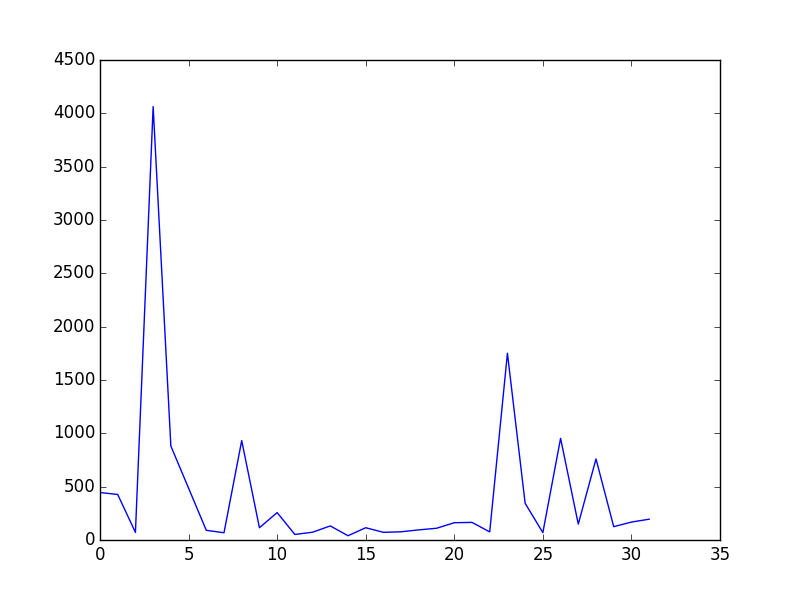
\includegraphics[scale=0.50]{CL_conferencePlagiarism.png}
\caption{Post Length for Article {\tt Conference Board Admits Plagiarism, Pulls Copyright Report}}

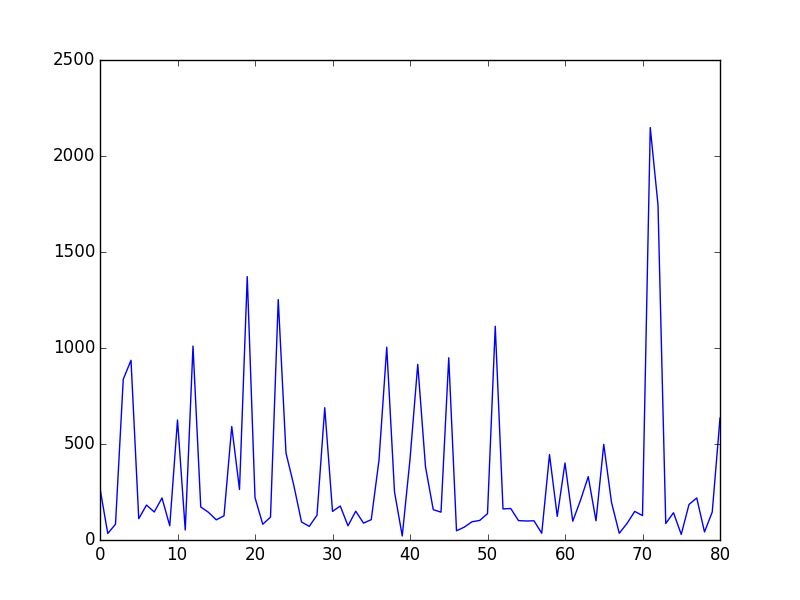
\includegraphics[scale=0.50]{CL_GooglesWave.png}
\caption{Post Length for Article {\tt Google's "Wave" Blurs Chat, Email, Collaboration Software}}
\end{center}
\end{figure}





One interesting preliminary result however, came from the metric of post length, and we look at the top 16 posters. We made plots of each user's post length and the conditional distribution of their post length when another user is in the same thread. There are several examples of these plots on subsequent pages.

\begin{figure}[here!]
\begin{center}
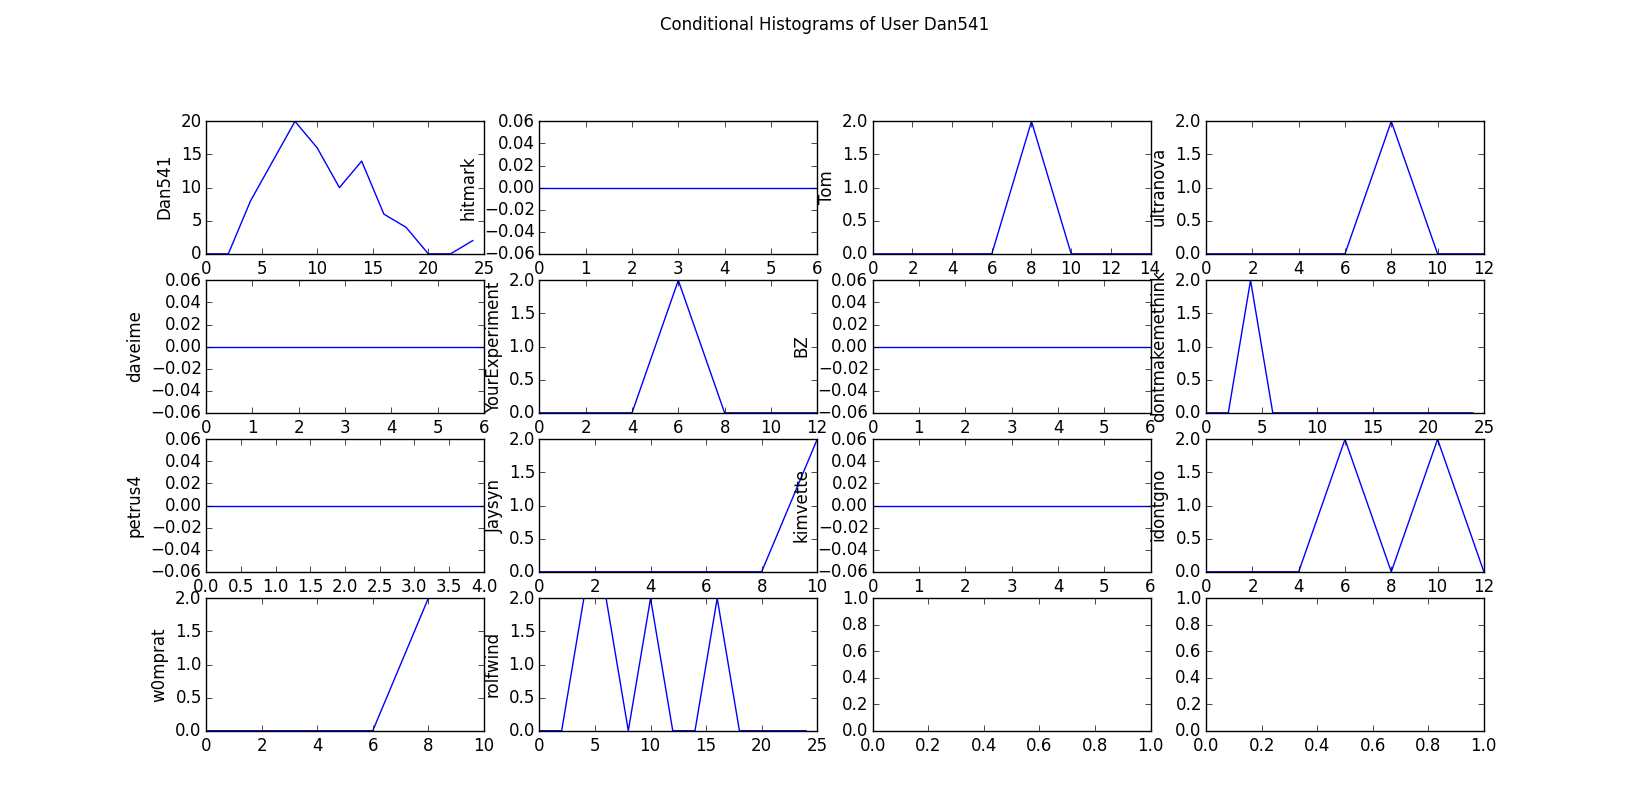
\includegraphics[scale=0.46, angle = 90]{Dan541.png}
\caption{Joint Distribution Plots for user {\tt Dan541} and Other Active User}
\end{center}
\end{figure}

\begin{figure}[here!]
\begin{center}
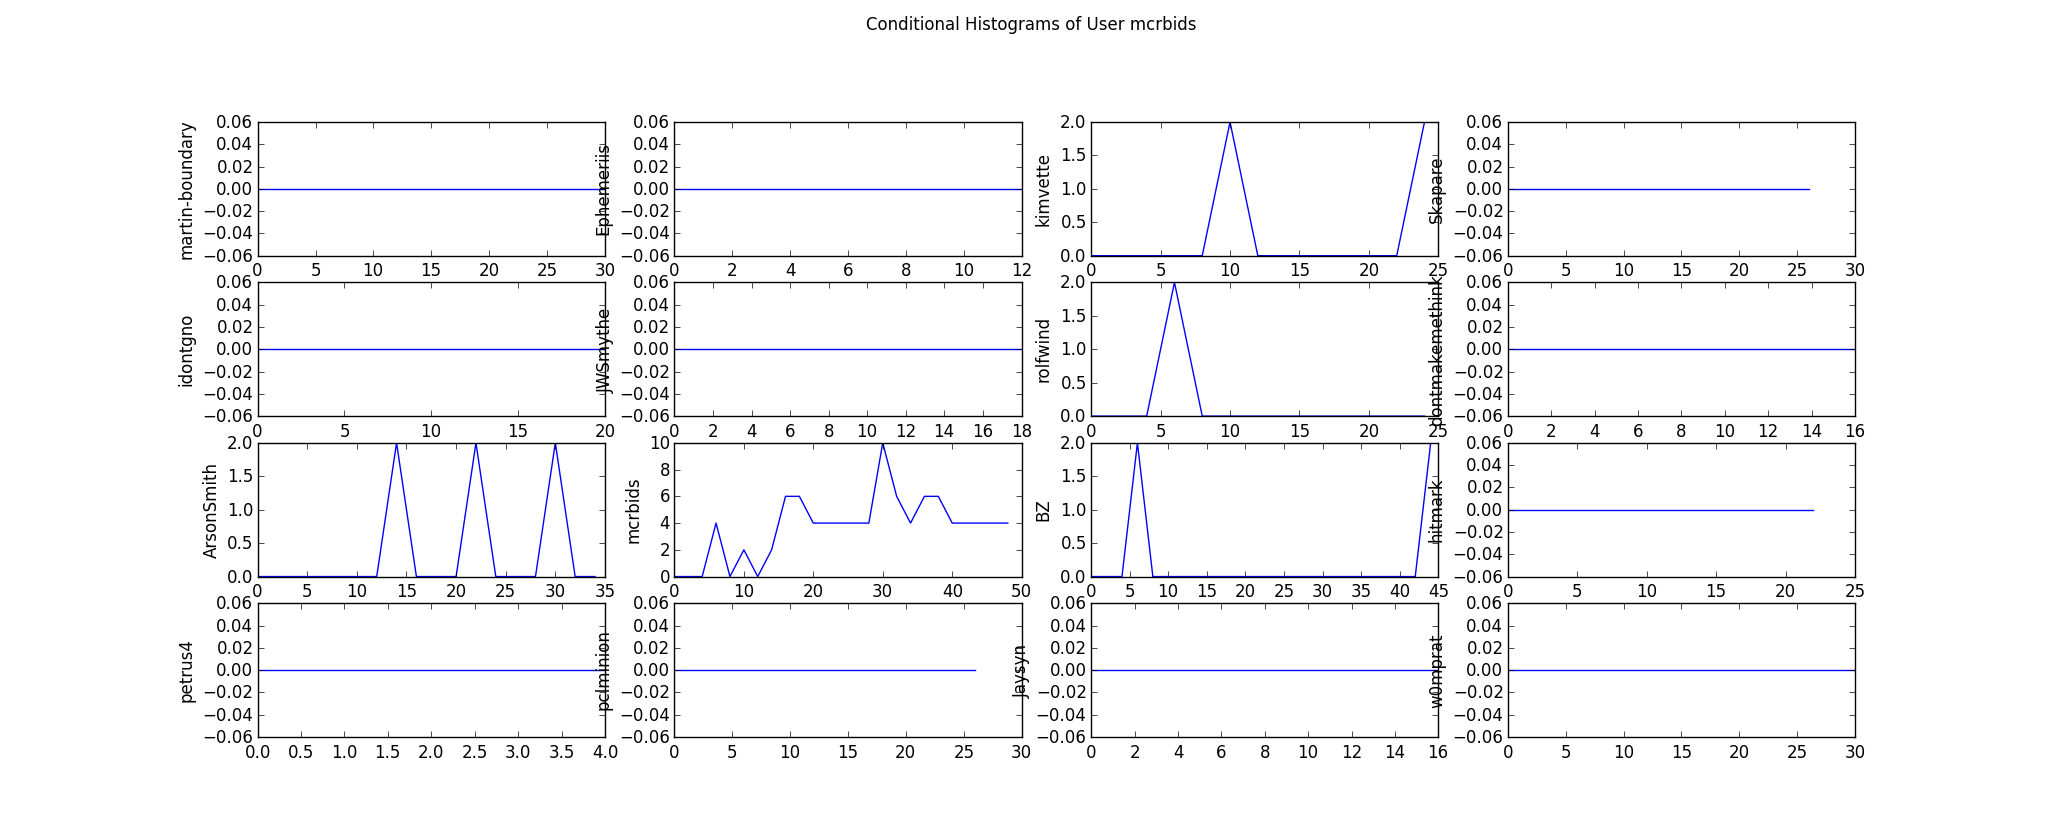
\includegraphics[angle = 90, scale=0.46]{mcrbids.png}
\caption{Joint Distribution Plots for user {\tt mcrbids} and Other Active User}
\end{center}
\end{figure}

Here, the $x$ axis denotes the square root of the number of characters in a post (we do this to scale down very long comment), and the $y$ axis denotes the number of threads for a given square root of comment length. The bin size for this histogram is $2$.

%We can see t

\subsubsection*{What we learnt}

%We have learnt that cleaning up of data takes a bit more time than expected. 

%I (Keegan) have also, learnt quite a fair bit of Python from Ben, as we have used Python exclusively. 
\begin{itemize}
%\item 
\item The comment length patterns differ significantly on the article. The next action item would be to learn the estimator based on a training sample. The features for this learning problem can be the length itself but can also be the content of the original post + first few comments.
\item Based on the conditional/joint distributions, we can see that users make differing lengths of posts depending on which particular user is in the conversation. However, this is for a small subset, and we want to see if this has any significance in a bigger set of data. 
\item A method to numerically compare the distribution to the conditional distribution will be very helpful. Chi square computation which we have not done is a good metric but we will need a larger dataset to see if there is any real pattern. 
\end{itemize}



\subsubsection*{Roles played}

Keegan - Analyzed data and co-author the report.  \\
Ben - Wrote code to do the plots and co-author the report.

\clearpage

\bibliographystyle{alpha}	
\bibliography{database}  % expects file "database.bib"
\end{document}




http://www.kuro5hin.org/story/2009/3/12/33338/3000
September 1st 2014

